We now give an overview of common data structures used in \BoxLib, followed by a simple
example written in both Fortran90 and C++ that makes use of these structures.
The example advances variables in time on multiple grids (no AMR) and produces plotfiles.

\section{Overview of Data Structures}

\BoxLib\ contains the most fundamental objects used to construct parallel
block-structured AMR applications.
At each level of refinement, the region covered by that level is divided
into grids, or boxes.  The entire computational domain is covered by
the coarsest (base) level of refinement (called level $\ell=0$ in C++ 
and called level $\ell=1$ in Fortran90) and can be represented on one
grid or divided into many grids.
Higher levels of refinement have cells that are finer by a ``refinement ratio''
of either 2 or 4.  The grids are properly nested in the sense that the union 
of grids at level $\ell+1$ is contained in the union of grids at level $\ell$.
Furthermore, the containment is strict in the sense that, except at physical 
boundaries, the level $\ell$ grids are large enough to guarantee that there is
a border at least $n_{\rm buffer}$ (typically $\sim$4) level $\ell$ cells wide surrounding each level
$\ell +1$ grid (grids at all levels are allowed to extend to the physical
boundaries so the proper nesting is not strict there).  See Figure \ref{fig:AMR}
for a sample two-dimensional grid structure.
As discussed earlier, the grids are distributed to processors in
a fashion designed to put roughly equal amounts of work on each
processor (load balancing).
%%%%%%%%%%%%%%%%%%%%%%%%%%%%%%%%%%%%%
\begin{figure}[tb]
\centering
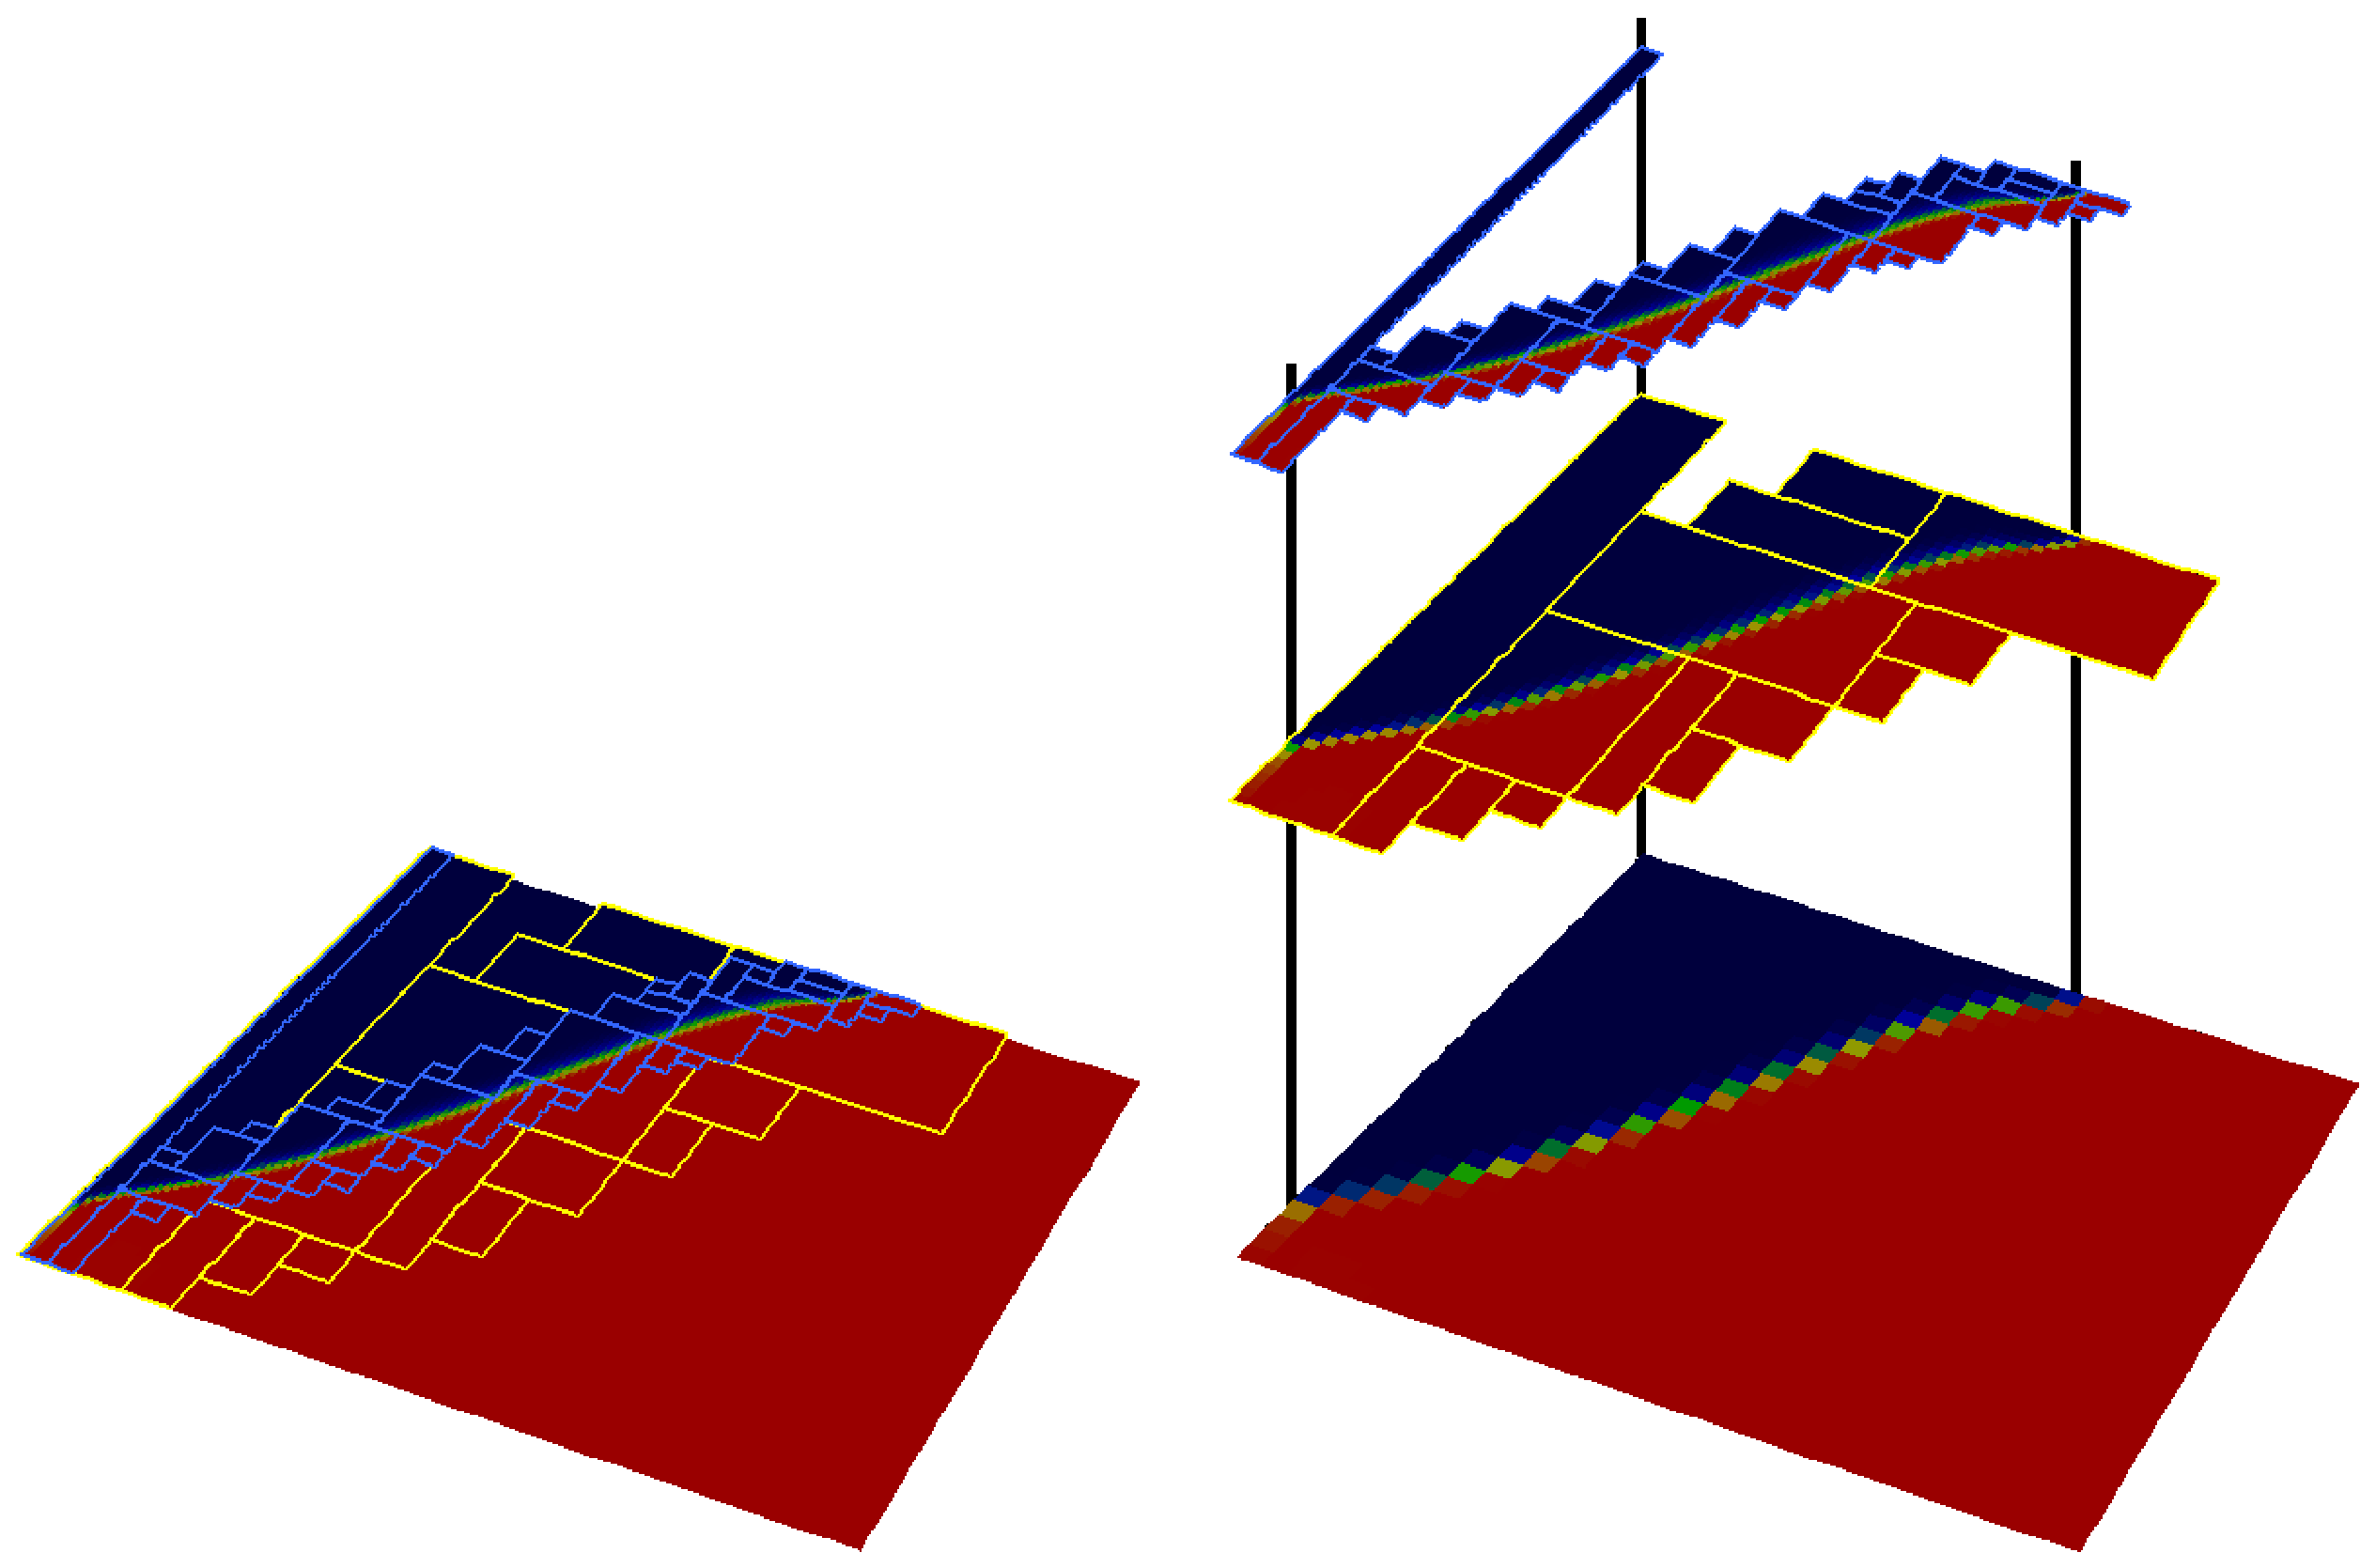
\includegraphics[width=6.5in]{./Introduction/AMR}
\caption{\label{fig:AMR}Sample grid structure with two levels of refinement.  These
grids satisfy the requirements that the base grid covers the entire computational domain 
and the grids are properly nested.  Note that refined grids are allowed to extend to the
domain boundary without coarser buffer cells.}
\end{figure}
%%%%%%%%%%%%%%%%%%%%%%%%%%%%%%%%%%%%%

On a grid, the data can be stored at cell-centers, faces, edges, or
corners (often called nodes).  In \BoxLib, data that is on an face is termed `nodal'
in that one direction (see Figure~\ref{fig:dataloc}).  In three-dimensions (not pictured),
data that is nodal in two directions is said to live on edges.  Data that is nodal in
all directions lives on the corners of cells.
\BoxLib\ uses $0$-based indexing, and for nodal data, the integer index
corresponds to the lower boundary in that direction.
In our \BoxLib\ applications, the state data (velocity, density, 
species, $\ldots$) is generally cell-centered.  Fluxes are typically nodal a
single direction (i.e.~they are face-centered).  A few quantities are nodal in all 
directions (e.g.~the pressure in the low Mach number projection methods).
%%%%%%%%%%%%%%%%%%%%%%%%%%%%%%%%%%%%%
\begin{figure}[tb]
\centering
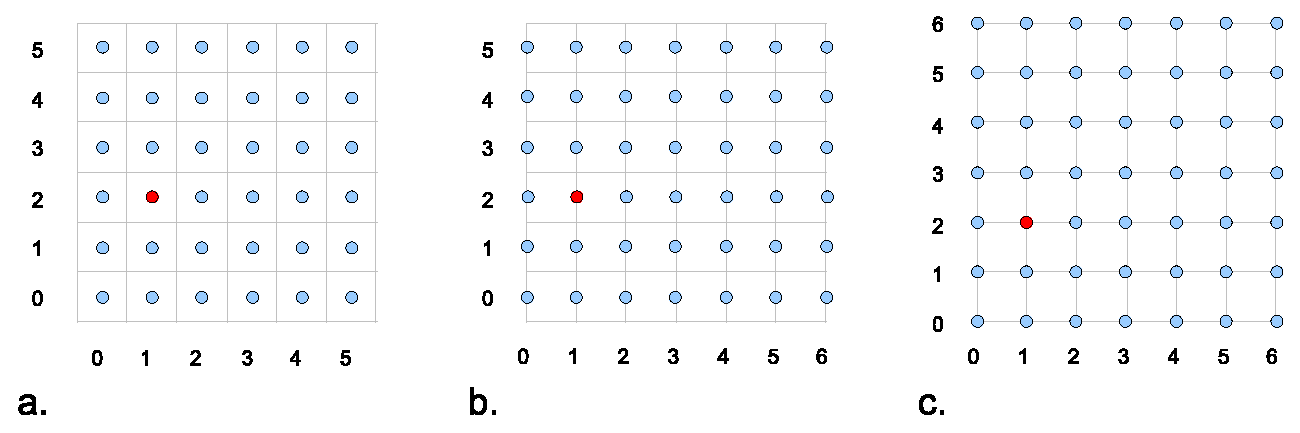
\includegraphics[width=6.5in]{./Introduction/data_loc2}
\caption{\label{fig:dataloc} Some of the different data-centerings in two dimensions:
(a) cell-centered, (b) nodal in the $x$-direction only (face-centered), and (c) nodal in
both the $x$- and $y$-directions.  Note that for nodal data, the
integer index corresponds to the lower boundary in that direction.
Also note that \BoxLib\ uses $0$-based indexing, e.g., in each of these centerings, 
the red point has the same indices:\ (1,2).
Not shown is the case where data is nodal in the $y$-direction only.  
Also not shown is the three-dimensional edge-centered case, where the data
is nodal in exactly two directions.  }
\end{figure}
%%%%%%%%%%%%%%%%%%%%%%%%%%%%%%%%%%%%%

\begin{itemize}
\item In C++ \BoxLib, we must specify the number of spatial dimensions (1, 2, or 3), 
{\tt DIM}, at compile-time.  The code that will be built is specifically designed to 
run only with that number of dimensions.
\item In Fortran90 \BoxLib, we build dimension-independent code at compile-time, 
and tell the program the dimensionality of the problem via a runtime inputs file.
\end{itemize}

To simplify the description of the underlying AMR grid, \BoxLib\
provides a number of classes.  We now briefly summarize some of the major
classes.

\subsection{\IntVect}

\IntVect s are {\tt DIM}-tuples of integers that are used to define
indices in space.  In C++, an example of an \IntVect\ in 2D would be
\begin{lstlisting}[backgroundcolor=\color{light-blue}]
IntVect iv(3,5);
\end{lstlisting}
In Fortran90, we don't use \IntVect\ s, but instead use standard
arrays of integers:
\begin{lstlisting}[backgroundcolor=\color{light-green}]
integer :: iv(2)
iv(1) = 3
iv(2) = 5
\end{lstlisting}

\subsection{\BoxType}

A \BoxType\ is simply a rectangular domain in space and does not hold any data.
A \BoxType\ contains the indices of its low end and high end, 
{\tt IntVect lo} and {\tt IntVect hi}.
\begin{itemize}
\item In C++, a \BoxType\ also
contains an {\tt IndexType} (cell-centered, face-centered, or nodal) for each
spatial direction.
\item In Fortran90, a \BoxType\ also contains the dimensionality 
of the \BoxType.
\end{itemize}
To build a \BoxType\ in C++ use:
\begin{lstlisting}[backgroundcolor=\color{light-blue}]
IntVect iv_lo(0,0);
IntVect iv_hi(15,15);
Box bx(iv_lo,iv_hi);
\end{lstlisting}
To build a \BoxType\ in Fortran90 use:
\begin{lstlisting}[backgroundcolor=\color{light-green}]
type(box) :: bx
integer   :: iv_lo(2), iv_hi(2)
iv_lo(1:2) = 0
iv_hi(1:2) = 15
bx = make_box(lo,hi)
\end{lstlisting}

The computational domain is divided into non-overlapping grids.  
The collection of grids at the same resolution comprise a level.
Figure~\ref{fig:boxes} shows three grids at the same level of
refinement.  Note that this figure cannot represent the base level of refinement,
since it would required that the grids span the problem domain.
The position of the grids is with respect to a global
index space at that level, and uses 0-based indexing.
For example, the \BoxType\ associated with grid 1 
in the figure has {\tt lo} = (2,6) and {\tt hi} = (5,13).
The global index space covers the entire domain at a given resolution.
For a simulation setup with 32 cells in each direction,
the coarsest level has $32 \times 32$ zones, and the
global index space will run from 0 to 31 in each coordinate
direction.  The next finer level will have a global index space running from 
0 to 63 in each coordinate direction (corresponding to $64 \times
64$ zones if fully refined), and the next finer level will have a global index
space running from 0 to 127 in each coordinate direction
(corresponding to $128\times 128$ zones if fully refined).
%%%%%%%%%%%%%%%%%%%%%%%%%%%%%%%%%%%%%
\begin{figure}[tb]
\centering
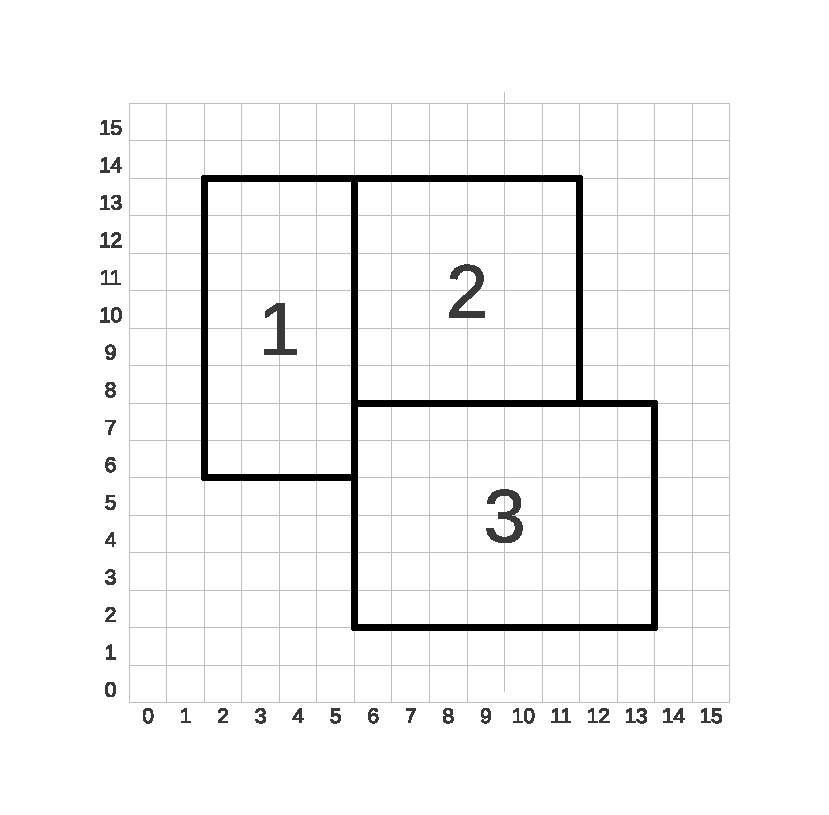
\includegraphics[width=4.0in]{./Introduction/index_grid2}
\caption{\label{fig:boxes} Three boxes that comprise a single level.
At this resolution, the domain is 16$\times$16 cells.}
\end{figure}
%%%%%%%%%%%%%%%%%%%%%%%%%%%%%%%%%%%%%

\subsection{\BoxArray}

A \BoxArray\ is an array of \BoxType es.  The size of the array is the 
number of \BoxType es in the \BoxArray.  Suppose your problem domain
has lo indicies (0,0) and hi indices (15,15), and you want to define
a \BoxArray\ to contain four $8\times 8$ boxes to cover the problem domain.
In Fortran90, you could do the following:
\begin{lstlisting}[backgroundcolor=\color{light-green}]
integer        :: lo(2), hi(2)
type(box)      :: bx(4)
type(boxarray) :: ba
lo(1) = 0
lo(2) = 0
hi(1) = 7
hi(2) = 7
bx(1) = make_box(lo,hi)
lo(1) = 8
lo(2) = 0
hi(1) = 15
hi(2) = 7
bx(2) = make_box(lo,hi)
lo(1) = 0
lo(2) = 8
hi(1) = 7
hi(2) = 15
bx(3) = make_box(lo,hi)
lo(1) = 8
lo(2) = 8
hi(1) = 15
hi(2) = 15
bx(4) = make_box(lo,hi)
call boxarray_build_v(ba,bx)
\end{lstlisting}
This is rather cumbersome, so instead we use other \BoxLib\ functions to
build the same \BoxArray:
\begin{lstlisting}[backgroundcolor=\color{light-green}]
type(boxarray) :: ba
integer        :: lo(2), hi(2)
type(box)      :: bx
lo(1:2) = 0
hi(1:2) = 15
bx = make_box(lo,hi)
call boxarray_build_bx(ba,bx)  ! the boxarray has one 16^2 box
call boxarray_maxsize(ba,8)    ! the boxarray has four 8^2 boxes
\end{lstlisting}
The analogous code in C++ is
\begin{lstlisting}[backgroundcolor=\color{light-blue}]
IntVect lo(0,0), hi(15,15);
Box bx(lo,hi);
BoxArray ba(bx);  // the BoxArray has one 16^2 box
ba.maxSize(8);    // the BoxArray has four 8^2 boxes
\end{lstlisting}

\subsection{\layout\ (Fortran90 Only)}

A \layout\ is a more intelligent \BoxArray, since it contains a \BoxArray\ as well
as the associated processor assignments, \BoxType\ connectivity, and many other
parallel constructs.  In the simplest case, if we have a \BoxArray\ {\tt ba} (obtained
from the example above), a 
\layout\ can be defined using:
\begin{lstlisting}[backgroundcolor=\color{light-green}]
type(layout) :: la
call layout_build_ba(la,ba)
\end{lstlisting}
In C++, the information that is contained in the Fortran90 \layout\ is part of
the \MultiFab\ class.

\subsection{\FArrayBox}

A \FArrayBox\ (or \Fab) is a ``Fortran array box'' that holds data.  It contains the
\BoxType\ that it is built on as well as a pointer to the data 
that can be sent to a Fortran routine.
In Fortran90, \Fab\ data is stored in a four-dimensional array,
{\tt (nx,ny,nz,nc)} in size, regardless of the dimensionality of the
problem.  Here {\tt nc} is the number of components, for instance
representing different fluid variables.  For 2D problems, {\tt nz=1}.

In \BoxLib, we don't usually deal with 
\Fab s alone, but rather through \MultiFab s, described next.

\section{The \MultiFab}
\MultiFab s are so important that we will give them their own section.
A \MultiFab\ is a collection of all the \Fab s at the same level of
refinement.
\begin{itemize}
\item In C++, a \MultiFab\ is defined using a \BoxArray,
number of components, and number of ghost cells that each \Fab\
will have.
\item In Fortran90, a \MultiFab\ is defined using a \layout,
number of components, , and number of ghost cells that each \Fab\
will have.
\end{itemize}
A \MultiFab\ has a ``valid'' region that is defined by 
the \BoxArray.  Each \Fab\ in the \MultiFab\ is built large enough 
to hold valid data and ghost cell data, and thus the \BoxType\ associated with
each \Fab\ is a grown version of the corresponding \BoxType\ from the \BoxArray.
Thus, a \Fab\ has no concept 
of ghost cells, it merely has a single \BoxType\ that identifies it.

To build a \MultiFab, we require a \layout\ (in Fortran90) or a \BoxArray\ (in C++).
In Fortran90, using the \layout\ built above, we build a \MultiFab\ using:
\begin{lstlisting}[backgroundcolor=\color{light-green}]
type(multifab) :: data
call multifab_build(data,la,2,6) ! build the multifab with 2 components 
                                 ! and 6 ghost cells

...                              ! do fun stuff with the data

call multifab_destroy(data)      ! free up memory to prevent leaks
\end{lstlisting}
In C++, using the \BoxArray\ built above, you could either build a \MultiFab, 
or a pointer to a \MultiFab:
\begin{lstlisting}[backgroundcolor=\color{light-blue}]
MultiFab* data = new MultiFab(ba,2,6);     // build pointer to MultiFab

...                                        // do fun stuff with the data

delete data;                               // free up memory
\end{lstlisting}

\subsection{Accessing Data}
Here is some sample Fortran90 code to access data within a \MultiFab:
\begin{lstlisting}[backgroundcolor=\color{light-green}]
integer                  :: i,dm,ng,nc,lo(2),hi(2)
type(multifab)           :: data
real(kind=dp_t), pointer :: dp(:,:,:,:)

...    ! build multifab data as described above

dm = data%dim   ! dm is dimensionality
ng = data%ng    ! ng is number of ghost cells
nc = data%nc    ! nc is number of components

do i=1,nboxes(data)
   ! if associated fab is not local to processor, then
   ! 'cycle', i.e., go to the next box
   if ( multifab_remote(data,i) ) cycle
   dp => dataptr(data,i)          ! dp points to data inside fab
   lo = lwb(get_box(data,i))      ! get lo indices of box
   hi = upb(get_box(data,i))      ! get hi indices of box
   select case(dm)
   case (2)
      call work_on_data_2d(dp(:,:,1,:), ng, nc, lo, hi)
   case (3)
      call work_on_data_3d(dp(:,:,:,:), ng, nc, lo, hi)
    end select
end do

! fill periodic domain boundary and neighboring grid ghost cells
call multifab_fill_boundary(data)  

...

subroutine work_on_data_2d(data, ng, nc, lo, hi)

  integer          :: lo(2), hi(2), ng
  double precision :: data(lo(1)-ng:,lo(2)-ng:,:)

  ! local variables
  integer :: i,j,n

  do j=lo(2),hi(2)
     do i=lo(1),hi(1)
        do n=1,nc
           ! some silly function I made up
           data(i,j,n) = (i + j) * n
        end do
     end do
  end do

end subroutine work_on_data_2d
\end{lstlisting}

In C++:
\begin{lstlisting}[backgroundcolor=\color{light-blue}]
#if    defined(BL_FORT_USE_UPPERCASE)
#define FORT_WORK_ON_DATA            WORK_ON_DATA
#elif  defined(BL_FORT_USE_LOWERCASE)
#define FORT_WORK_ON_DATA            work_on_data
#elif  defined(BL_FORT_USE_UNDERSCORE)
#define FORT_WORK_ON_DATA            work_on_data_
#endif

extern "C"
{
    void FORT_WORK_ON_DATA (
        Real* data, const int* Ncomp, const int* ng,
        const int* lo, const int* hi);
}

int main()
{
  int Ncomp = 2, Nghost = 6;

  ...    // build pointer to MultiFab* data as described above
  
  // MFIter is a ``MultiFab Iterator'' that essentially
  // loops over grids
  for ( MFIter mfi(*data); mfi.isValid(); ++mfi )
  {
    const Box& bx = mfi.validbox();
    FORT_WORK_ON_DATA((*data)[mfi].dataPtr(),
                      bx.loVect(), bx.hiVect(), &Ncomp, &Nghost);
  }
  // fill periodic domain boundary and neighboring grid ghost cells
  data->FillBoundary();
}
\end{lstlisting}
The {\tt FORT\_WORK\_ON\_DATA} calls a Fortran90 subroutine which is nearly
identical to the example given above.  The only difference is the subroutine
name cannot have the \_2d or \_3d in its name.  Thus, the 2d and 3d versions
are both named {\tt subroutine work\_on\_data}, and must be written in
different .f90 files.


\subsection{Other \MultiFab\ Functions}
{\tt setVal} is a simple subroutine that sets the \MultiFab\ data to a particular value.
In Fortran90, use:
\begin{lstlisting}[backgroundcolor=\color{light-green}]
! set all variables to 0.0; ``all=.true.'' means set the ghost cells also
call setval(data,0.d0,all=.true.)
\end{lstlisting}
In C++, use:
\begin{lstlisting}[backgroundcolor=\color{light-blue}]
data->setVal(0.0);  // set all variables to 0.0, including ghost cells
\end{lstlisting}
{\tt copy} is a simple subroutine that copies data from one \MultiFab\ to another.
In Fortran90, use:
\begin{lstlisting}[backgroundcolor=\color{light-green}]
! copy components 1 and 2 from data_src into data_dest, 
! including the ghost cells. calling sequence is 
! (1) destination multifab, (2) first component of destination, 
! (3) source multifab, ! (4) first component of source, 
! (5) number of components, (6) ghost cells
call multifab_copy_c(data_dest,1,data_src,1,2,6)
\end{lstlisting}
In C++, use:
\begin{lstlisting}[backgroundcolor=\color{light-blue}]
// copy components 0 and 1 from data_src into data_dest, 
// including the ghost cells. calling sequence is 
// (1) destination multifab, (2) source multifab, 
// (3) first component of destination, (4) first component of source, 
// (5) number of components, (6) ghost cells
MultiFab::Copy(data_dest,data_src,0,0,2,6)
\end{lstlisting}
There are many other subroutines available for adding, subtracting, multiplying, etc.,
components of \MultiFab s, finding the min/max value, norms, number of cells, etc.
Refer to {\tt BoxLib/Src/F\_BaseLib/multifab\_f.f90} or 
{\tt BoxLib/Src/C\_BaseLib/MultiFab.H} for a complete listing.

\section{Simple Example - Fortran90}
We now present a complete sample code that uses the concepts discussed up to this point.
The example also writes plotfiles that can be viewed, and can be run in parallel if you
are working on a machine with MPI.  The Fortran90 version of this example is contained in 
{\tt BoxLib/Tutorials/WaveEquation\_F/}.

In this example, we advance the equations:
\begin{eqnarray}
\frac{\partial\phi_1}{\partial t} &=& \phi_2, \\
\frac{\partial\phi_2}{\partial t} &=& \nabla^2\phi_1,
\end{eqnarray}
on a domain from -1 to 1 in each spatial direction with initial conditions
\begin{eqnarray}
\phi_1(t=0) &=& 0 \\
\phi_2(t=0) &=& e^{-100r^2},
\end{eqnarray}
where $r$ is the distance from the cell-center to the center of the domain.
We use uniform grid spacing in each direction, i.e., $\Delta x = \Delta y = \Delta z$,
and for this example, we used a fixed time step with $\Delta t = 0.1\Delta x$.
To advance these equations, we use a Runge-Kutta temporal discretization and a 
fourth-order spatial discretization of the Laplacian.  This example does not use AMR, 
and uses periodic boundary conditions on all sides.

In the problem directory, you will see the following files:
\begin{itemize}
\item {\tt GNUmakefile}

This contains compiler settings and directories required by the make system to build the code.

  \begin{itemize}

    \item {\tt BOXLIB\_HOME}

    Change this to point to the \BoxLib\ home directory.  Alternatively, you can define {\tt BOXLIB\_HOME}
    as an environment variables on your system.

    \item {\tt NDEBUG} ('{\tt t}' or '{\tt f}')
      
    ``not debug'' (we know, confusing).  If '{\tt t}', modifies compiler flags to build a 
    more optimized version of the code.  The program will run faster, but have fewer 
    runtime error checks.

    \item {\tt MPI} ('{\tt t}' or '{\tt f}')

    Indicate whether you want your executable to be MPI-compatible.  MPI must be installed on your
    machine in order to use this.

    \item {\tt OMP} ('{\tt t}' or '{\tt f}')

    Turns on OpenMP compiler flags.  Note that you still must write OpenMP directives into your code.

    \item {\tt PROF} ('{\tt t}' or '{\tt f}')

    Turns on timer compilation flags.  Timers are useful for optimizing your code since they tell you 
    what subroutines are taking the most time and require more optimization.  Note that you still have 
    to write timers into your code.

    \item {\tt COMP} ('{\tt gfortran}, {\tt Intel}, $\ldots$)'

    The Fortran compiler.  Supported options include {\tt gfortran}, {\tt Intel}, {\tt PathScale}, and 
    {\tt PGI}.  The {\tt gfortran} compiler seems to 
    be bug-free on all systems we've run on.  {\tt Intel} after version 9 seems flaky.  {\tt PathScale} 
    (available at OLCF and NERSC) seems to work as long as you don't turn the optimization flags too high.
    {\tt PGI} (available at OLCF and NERSC) seems to work fine, but is slower than the others.

    \item {\tt MKVERBOSE} ('{\tt t}' or '{\tt f}')

    Verbosity of compile-time output.

  \end{itemize}

\item {\tt GPackage.mak}

List of local files needed to be included in the build.  The {\tt GNUmakefile} points to this.

\item {\tt main.f90}, {\tt init\_data.f90}, {\tt advance.f90}, {\tt write\_plotfile.f90}

Source code that is not within the {\tt BoxLib/Src/} tree.  Note: if a file that exists in the
{\tt BoxLib/Src/} tree also exists in the local directory, the local copy takes precedence.
{\tt main.f90} is the main driver.

\item {\tt inputs\_2d}, {\tt inputs\_3d}

Inputs files to customize the simulation parameters.

\end{itemize}

To build the code, simply type ``{\tt make}''.  An exectubale will appear that has some indication (but not complete)
about what setting you used in the {\tt GNUmakefile}.  To run the code serially, simply type, for example,
\begin{lstlisting}[backgroundcolor=\color{light-red}]
./main.Linux.gfortran.exe inputs_2d
\end{lstlisting}
The program will complete and there will be a series of plotfiles, e.g., {\tt plt00000}, in the run directory.
You can open these using {\tt VisIt} (available at {\tt https://wci.llnl.gov/codes/visit/}) by opening
the {\tt Header} file within the plotfile directory.  (For the {\tt VisIt} novice, after you open the {\tt Header}
file, select ``Add'' $\rightarrow$ ``Pseudocolor'' $\rightarrow$ ``Variable 2'' and then click ``Draw''.)

\section{Simple Example - C++}
The C++ version of this example is contained in {\tt BoxLib/Tutorials/WaveEquation\_C/}.

\begin{itemize}
\item {\tt GNUmakefile}

This contains compiler settings and directories required by the make system to build the code.

  \begin{itemize}

    \item {\tt BOXLIB\_HOME}

    Change this to point to the \BoxLib\ home directory.  Alternatively, you can define {\tt BOXLIB\_HOME}
    as an environment variables on your system.

    \item {\tt DEBUG} ('{\tt TRUE}' or '{\tt FALSE}')
      
    Debug mode.  If 'FALSE', modifies compiler flags to build a more optimized version of the code.
    The program will run faster, but have fewer runtime error checks.

    \item {\tt USE\_MPI} ('{\tt TRUE}' or '{\tt FALSE}')

    Indicate whether you want your executable to be MPI-compatible.  MPI must be installed on your
    machine in order to use this.

    \item {\tt USE\_OMP} ('{\tt TRUE}' or '{\tt FALSE}')

    Turns on OpenMP compiler flags.  Note that you still must write OpenMP directives into your code.

    \item {\tt PROFILE} ('{\tt TRUE}' or '{\tt FALSE}')

    Turns on timer compilation flags.  Timers are useful for optimizing your code since they tell you 
    what subroutines are taking the most time and require more optimization.  Note that you still have 
    to write timers into your code.

    \item {\tt COMP} ('{\tt g++}, {\tt Intel}, $\ldots$)'

    The C++ compiler.  Supported options include {\tt g++}, {\tt Intel}, {\tt PathScale}, and 
    {\tt PGI}.  The {\tt g++} compiler seems to 
    be bug-free on all systems we've run on.  {\tt Intel} after version 9 seems flaky.  {\tt PathScale} 
    (available at OLCF and NERSC) seems to work as long as you don't turn the optimization flags too high.
    {\tt PGI} (available at OLCF and NERSC) seems to work fine, but is slower than the others.

    \item {\tt FCOMP} ('{\tt gfortran}, {\tt Intel}, $\ldots$)'

    The Fortran compiler.  Supported options include {\tt gfortran}, {\tt Intel}, {\tt PathScale}, and 
    {\tt PGI}.  The {\tt gfortran} compiler seems to 
    be bug-free on all systems we've run on.  {\tt Intel} after version 9 seems flaky.  {\tt PathScale} 
    (available at OLCF and NERSC) seems to work as long as you don't turn the optimization flags too high.
    {\tt PGI} (available at OLCF and NERSC) seems to work fine, but is slower than the others.

    \item {\tt DIM} (1', '2', or '3')

    Dimensionality of the problem.  Unlike Fortran90, you need to set this in the C++ version.

    \item {\tt PRECISION} ('{\tt DOUBLE}' or '{\tt FLOAT}')

    Precision of real numbers.  You can use {\tt FLOAT} for single-precision real numbers to save memory.

    \item {\tt EBASE} ('{\tt main}', $\ldots$)

    The executable string will begin with this.

  \end{itemize}

\item {\tt Make.package}

List of local files needed to be included in the build.  The {\tt GNUmakefile} points to this.

\item {\tt main.f90}, {\tt writePlotFile.cpp}, {\tt writePlotFile.H}, {\tt init\_data\_2d.f90},
      {\tt init\_data\_3d.f90}, {\tt advance\_2d.f90}, {\tt advance\_3d.f90}

Source code that is not within the {\tt BoxLib/Src/} tree.  Note: if a file that exists in the
{\tt BoxLib/Src/} tree also exists in the local directory, the local copy takes precedence.
{\tt main.f90} is the main driver.

\item {\tt inputs\_2d}, {\tt inputs\_3d}

Inputs files to customize the simulation parameters.

\end{itemize}

To build the code, simply type ``{\tt make}''.  An exectubale will appear that has some indication (but not complete)
about what setting you used in the {\tt GNUmakefile}.  To run the code serially, simply type, for example,
\begin{lstlisting}[backgroundcolor=\color{light-red}]
./main2d.Linux.g++.gfortran.ex inputs_2d
\end{lstlisting}
The program will complete and there will be a series of plotfiles, e.g., {\tt plt00000}, in the run directory.
You can open these using {\tt VisIt} (available at {\tt https://wci.llnl.gov/codes/visit/}) by opening
the {\tt Header} file within the plotfile directory.  (For the {\tt VisIt} novice, after you open the {\tt Header}
file, select ``Add'' $\rightarrow$ ``Pseudocolor'' $\rightarrow$ ``Variable 2'' and then click ``Draw''.)

\section{Running in Parallel}
We will now demonstrate how to run the example in {\tt BoxLib/Tutorials/WaveEquation\_C/}
in parallel.  On your local machine, if you have MPI installed, you can simply build
the executable as describe before, but with {\tt USE\_MPI=TRUE} in the {\tt GNUmakefile}.
Alternatively, you can override the settings in {\tt GNUmakefile} at the command line
using, e.g., ``{\tt make USE\_MPI=TRUE}''.  
An executable named {\tt main2d.Linux.g++.gfortran.MPI.ex} will be built.
Then you can run the program in parallel using, e.g.,
\begin{lstlisting}[backgroundcolor=\color{light-red}].
mpiexec -n 4 main2d.Linux.g++.gfortran.MPI.ex inputs_2d
\end{lstlisting}

To run in parallel on the hopper machine at NERSC, first copy the \BoxLib\ source code
into your home directory on hopper and enter the {\tt WaveEquation\_C/} directory.
The default programming environment uses the {\tt PGI} compilers, so we will switch to the
{\tt gnu} programming environment to make {\tt g++} and {\tt gfortran} available
using the command:
\begin{lstlisting}[backgroundcolor=\color{light-red}].
module swap PrgEnv-pgi PrgEnv-gnu
\end{lstlisting}
Next, in {\tt GNUmakefile}, set {\tt USE\_MPI=TRUE}, and then type ``{\tt make}''
(or alternatively, type ``{\tt make USE\_MPI=TRUE}'').
An executable named {\tt main2d.Linux.g++.gfortran.MPI.ex} will be built.
You cannot submit jobs in your home directory, so change to a scratch space
(``{\tt cd \$SCRATCH}'' will typically do), and copy the executable and
{\tt inputs\_2d} into this directory.  Then you need to create a job script,
e.g., "{\tt hopper.run}", that has contents:
\lstinputlisting[backgroundcolor=\color{light-red}]{./GettingStarted/hopper.run}
To run, simply type ``{\tt qsub hopper.run}''.  You can monitor the status of your job
using ``{\tt qstat -u <username>}'' and view your position in the queue 
using ``{\tt showq}''.
